\chapter{基于SDN的云平台架构设计}
基于SDN的云平台多租户虚拟网络定制化的研究,主要是将SDN集中控制和可编程的优势,集成到云数据中心,通过网络虚拟化技术,为租户提供相互隔离的vSDN网络,vSDN网络由租户自由的控制器实现集中管控。物理网络的集中管控,方便运营商对数据中心网络的管理和维护;租户vSDN网络的集中控制,便于租户利用自己的控制期开发适合自己的上层应用。本章最该研究的主要架构进行简单的介绍。
\section{关键技术分析}
\subsection{需求分析}
基于SDN的云平台多租户虚拟网定制化的实现,首先解决的是物理网络资源的虚拟化,其次是在虚拟化的基础上进行虚拟网络的带宽时延测量,随后根据测量的带宽时延进行链路的定制化,最后为方便用户的操作,完成前端Web界面的设计和实现。

系统的整体需求如图\ref{fig:ovx}所示。

\begin{figure}[!htb]
  \centering
  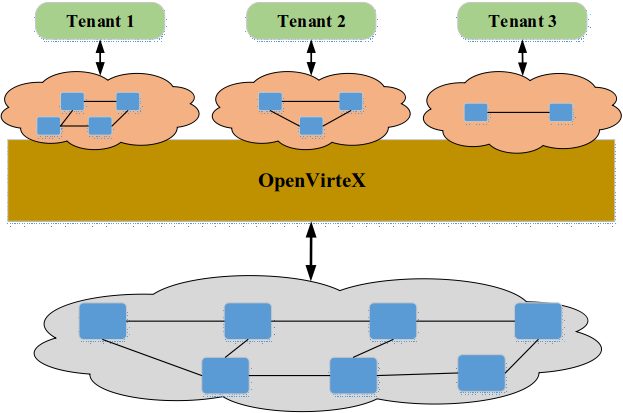
\includegraphics[width=0.7\textwidth]{logo/ovx.png}
  \caption{OVX网络虚拟化示意图}
  \label{fig:ovx}
\end{figure}

网络的虚拟化,需要实现资源隔离的同时,还要满足虚拟网络支持SDN模式,本文选用支持资源虚拟化的SDN控制器来完成该功能,通过对底层物理网络中下发的流表信息中,添加租户ID的相关信息,完成底层网络中租户的隔离工作。通过自身维护的物理网络与虚拟网络的映射关系图,为上层SDN交换机提供支持OpenFlow协议的虚拟网络,此时租户便可利用自身的SDN控制器完成对vSDN网络的集中管控。

在虚拟资源之上进行链路带宽时延等信息的测量工作,需要实现SDN模式下链路的带宽、时延的精确测量,由于SDN的集中控制和可编程的先天优势,控制器端可以看到全局的网络拓扑,与此同时,OpenFlow协议的规范性和便捷性,方便了我们实现可用带宽、已用带宽、时延的精确测量工作,测量的数据成为用户做出决策的考量值。

链路的定制化,需要用户根据链路的时延、带宽等信息,选取便于传输的最优链路,进行定制化流表的下发工作,此时,租户便可以对自己在数据中心的虚拟机,进行远程的操控,可以自定义数据的传输路径。

前端的Web界面方便了用户的操作,用户可以在其web界面,通过简单的点击操作,完成对数据中心网络的定制化操作。包括物理、虚拟网络的拓扑获取,链路带宽、时延的前端展示,虚拟网络的创建,定制化链路的前端选取等功能。一系列的操作,需要实现租户之间的隔离工作,我们需要通过认证功能,对租户的请求进行认证。实现租户操作的隔离行。

\subsection{关键技术}
本文旨在构建一个基于SDN的云平台多租户虚拟网络定制化的平台,该平台一方面实现对云平台数据中心网络的集中控制,方便运营商对数据中心网路的管理和运维,加快了新业务的引入速度,运营商可以通过可控的软件部署相关的功能,该自动化部署和运维故障诊断,减少了网络的人工干预,降低了网络的运营费用,也降低了出错率。与此同时,通过虚拟化技术,基于底层的统一物理资源,虚拟出相互隔离的租户vSDN网络,vSDN网络由租户自己的SDN控制器实现集中管控,实现了租户对数据中心网络的集中管控,租户可以为自己的控制器开发特有的北向应用,从而定制化数据中心业务需求,当然租户对数据中心虚拟网络的集中管控,可以实现租户对自有网络的监控工作,并可根据当前负载定制化链路的转发路径。为实现上述功能,需要突破以下关键技术。

\begin{enumerate}
\item 基于SDN的云平台系统搭建。将SDN集成到云平台数据中心,系统的搭建尤为重要,如何在实现相应功能,满足租户需求的情况下,搭建一套性能稳定的系统成为本文的关键所在。为此,本文创新性地提出了基于SDN的云平台多租户虚拟网络定制化机制,在实现对数据中心网路集中控制的同时,利用虚拟化技术虚拟出相互隔离的vSDN网络,该网路由租户自有的控制器实现集中管控,这样,租户便可以利用自己的SDN控制器完成对自有网络的灵活控制。为方便与OpenStack云平台的集成,本文在对OpenStack云平台改动最小、性能降低最低的情况下,完成了整体系统的搭建,系统将虚拟化平台与OpenStack内部的网络模块Neutron分工合作,Neutron主要负责OpenStack内部网络资源的管理和控制,而本文中支持SDN模式的虚拟化平台主要负责物理服务器之间的物理网络的管理和控制,两者协同工作,共同完成SDN与OpenStack的集成工作,开放控制器给租户,实现租户对数据中心虚拟网络的灵活管控。
\item 链路带宽、时延测量。SDN控制器开发给租户后,利用SDN控制器实现对vSDN网络的负载情况的精确测量,是每一个租户希望看到的,测量数据的精确性,直接决定了数据转发策略的制定。因此,全局网络的带宽、时延数据的测量,在本文中起到关键作用。针对带宽、时延,本文创新性地提出了SDN模式下的测量方法。首先针对链路可用带宽,本文采用包对技术,精确地测量了链路的可用带宽,测试证明,该方法在低带宽模式下具有精确的测量结果。针对时延,本文基于三点模式的数据报传输,通过统计时间差的模式,完成了数据的精确测量。带宽和时延数据,成为了租户进行链路定制化的重要依据,租户根据当前链路的负载情况,可以选取一条最优的链路进行数据的传输,在提高数据中心带宽利用率的同时,极大地提高了租户网络的数据传输速率。
\end{enumerate}

\section{系统架构设计}
\subsection{系统总体设计图}
系统主要由四个模块组成。分别为网络虚拟化模块、控制器模块、通信模块和GUI模块。总体的架构图如图\ref{fig:ovx}所示。

\begin{figure}[!htb]
  \centering
  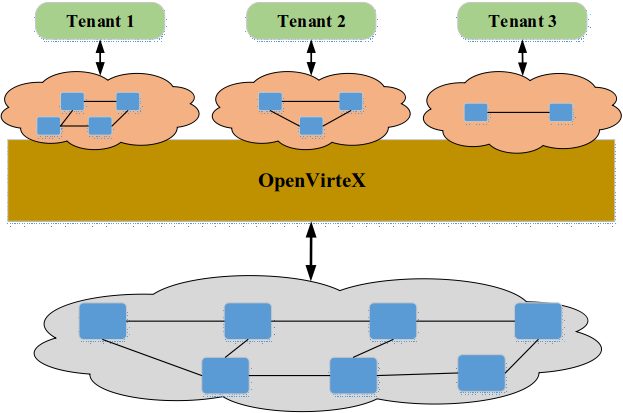
\includegraphics[width=0.7\textwidth]{logo/ovx.png}
  \caption{OVX网络虚拟化示意图}
  \label{fig:ovx}
\end{figure}

如图中所示,架构底层主要包含支持OpenFlow协议的交换机,以及OpenStack内部的虚拟机资源,交换机既包含OpenStack内部的虚拟网桥,亦包含连接物理服务器之间的物理OpenFlow交换机。将这部分网络开放给租户,主要是为了便于租户实现对数据中心物理网络的可控性。租户可以根据链路时延、带宽定制化最优数据传输链路。支持网络虚拟化的SDN控制器,实现对底层网络和计算资源的集中控制。由该模块,可以创建相互隔离的租户虚拟网络,该虚拟网络支持SDN模式,租户可利用控制器实现对自由虚拟网络的集中管控。自主开发北向应用,实现特有的功能。

控制器模块主要实现对租户控制器的管理。租户的控制器实现对自有vSDN网络的集中管控,该控制器运行于特定虚拟机之中,租户可以登录虚拟机,进行相应的配置和开发工作。每一个vSDN网络对应唯一的SDN控制器。现有的控制器镜像,已经开发了对链路带宽、时延的测量功能,租户可以登录控制器所在的虚拟机,开发自己的北向应用。

通信模块主要实现异步通信,前端对网络拓扑的获取、带宽时延数据的获取以及虚拟网络的创建请求,均通过通信模块,分别和控制器、网络虚拟化模块完成数据的请求和获取。通信模块完成了进程间的异步通信。

前端GUI界面,主要为了方便用户的操作,用户可以在其web界面,通过简单的点击操作,完成对数据中心网络的定制化操作。包括网络拓扑的显示,链路带宽、时延的前端展示,虚拟网络的创建操作,定制化链路的前端选取等功能。前端模块的极大的提高了用户体验效果。

\subsection{系统详细架构图}
在OpenStack云平台数据中心网络中采用SDN架构,核心思想是用控制器对网路运营模式实现统一管控。现有云数据中心网络的模式均为单一节点控制,该模式下的SDN网络对于租户是不可见的。本文提出了多租户虚拟化网络的定制和管理方案,实现了租户自有控制器对虚拟网络的灵活控制。多租户对应多控制器的机制便于租户对自有网络进行带宽时延查询、定制化流表下发、链路切换、控制器北向接口开发实验等自定义操作。系统的详细架构图如图\ref{fig:architecture}所示。

\begin{figure}[!htb]
  \centering
  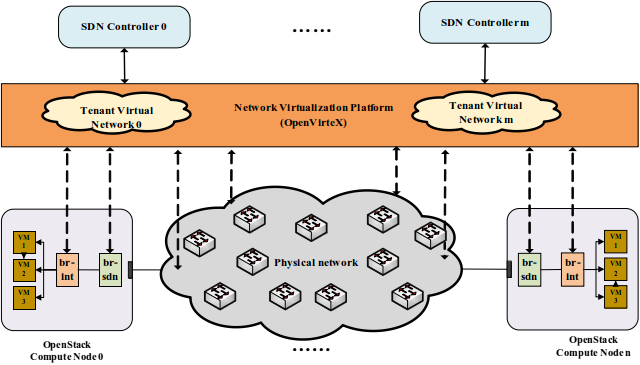
\includegraphics[width=0.7\textwidth]{logo/architecture.png}
  \caption{系统详细架构图}
  \label{fig:architecture}
\end{figure}

在兼容现有OpenStack网络模式的前提下,为OpenStack平台的每个计算节点添加br-sdn网桥,由于br-int网桥实际就是一个NORMAL交换机,不管其受SDN控制器控制与否,不会影响其作用,故我们将该网桥以及连接物理服务器之间的支持OpenFlow协议的交换机均受OVX控制器进行管控,OVX控制器实现对网络的集中控制,与此同时,OVX支持SDN模式下的网络虚拟化,可以虚拟出相互隔离的vSDN网络,vSDN网络由租户自己的控制器进行集中控制。前端GUI模块基于OpenStack的Horizon模块进行二次开发,为其添加两个Panel,分别实现对物理网络和虚拟网络的拓扑展示,全局链路带宽、时延展示,以及虚拟网络创建和删除的前端操作。

在该架构图中,OVX与OpenStack中的Neutron组件并列存在,Neutron主要管控OpenStack内部的虚拟网络,包括各种防火墙、router、DNS服务,而OVX主要负责连接服务器之间的物理网络的连接状态。两者并列存在。相互协同工作。这种实现的模式可以在对OpenStack云平台改动最小、性能影响最低的情况下完成SDN与OpenStack的集成。

对于数据传输,现有架构下,有两种模式可以选择。租户可以选择使用传统网络模式进行数据的传输,数据经br-int和br-tun,由传统模式交换机,进行数据的传输。与此同时,租户亦可通过流表的下发,实现SDN模式下的数据传输,该模式下,数据经由br-int和br-sdn,途径支持OpenFlow协议的交换机,完成数据的转发工作。两种模式的并存,租户可以自主选择切换模式。现有的SDN模式,相比于传统模式,SDN模式下租户可以开发自己的北行应用,实现数据中心网络的相关功能的自定义。当然SDN现有模式仅仅实现了二层转发,跨路由的传输现阶段只能通过传统模式实现。

\subsection{系统流程图}
系统的整体流程图如图\ref{fig:workflow}所示。流程图主要对系统整体的工作流进行了阐述。详细讲解了从虚拟网络创建到链路定制化的整个流程。

\begin{figure}[!htb]
  \centering
  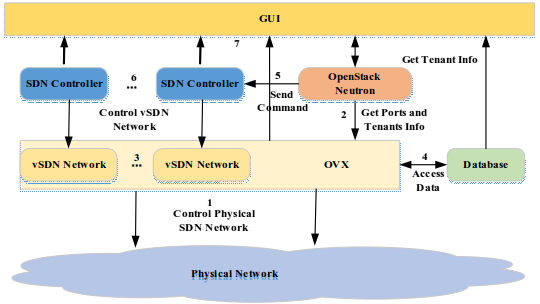
\includegraphics[width=0.7\textwidth]{logo/workflow.png}
  \caption{系统详细流程图}
  \label{fig:workflow}
\end{figure}

\begin{enumerate}
\item 网络虚拟化平台OVX实现对底层物理网络管理,完成物理网络的集中控制。本研究为其开发了创建虚拟网络的API接口createCustomNetwork,租户可以调用该接口,实现虚拟网络的创建。OVX自身维护虚拟网络与物理网络的映射表,完成南北向指令的映射工作。
\item 从OpenStack Neutron侧,获取虚拟机以及虚拟机绑定br-int网桥的端口信息,OVX本身只能获取到交换机的连接信息,两者结合,得到全网的完整拓扑信息图。基于此物理网络信息,进行虚拟网路的创建。
\item 本研究对OVX封装了创建虚拟网路的createCustomNetwork接口,调用该API接口,完成虚拟网络的创建。该虚拟网络基于底层的物理资源,可以是底层物理资源的同构子图,也可以是自定义的虚拟网络拓扑图。
\item 在网络虚拟化平台OVX侧,每个虚拟网络由\emph{virtualnetworkid}进行标识。在OpenStack中,每个租户有自己的ID号\emph{tenantid}。本文将两者的对应关系存储到数据库中。另外,对创建的虚拟网络以及虚拟网络和物理网络的对应关系,亦存储到数据库中,方便用户进行数据的读取和修改。本研究采用MongoDB数据库完成上述操作。由于MongoDB为非关系型数据库,处理json格式的数据非常便捷。
\item OpenStack Neutron侧发送指令到SDN控制器。现阶段,指令主要包括带宽/延迟测量以及定制化流表的下发。未来我们的平台将提供更多的功能。
\item SDN控制器接收到消息,通过我们开发的应用,完成相应的测量工作。最后返回对应的数据。租户可以登录到SDN控制器所在的虚拟机,开发自己的应用程序,以实现更多的功能。
\item GUI界面完成物理网络、虚拟网络、链路带宽、时延等信息的获取,在前端界面完成展示工作。
\end{enumerate}

\section{模块详解}
\subsection{网络虚拟化模块}
网络虚拟化允许不同需求的用户组访问同一个物理网络,但从逻辑上对它们进行一定程度的隔离,以确保安全。凭借网络虚拟化技术,能在单一物理基础设施上部署多个封闭用户组,并在整个网络中保持高标准的安全性、可扩展性、可管理性和可用性。通过网络虚拟化可实现弹性、安全、自适应、易管理的基础网络,充分满足服务器虚拟化等虚拟技术对基础网络带来的挑战,达到提高数据中心的运行效率、业务部署灵活、降低能耗、释放机架空间的目的。

本文选用的网络虚拟化平台,通过给每个租户提供访问一个虚拟网络拓扑和一个完整的网络头空间来完成虚拟网络的创建,呈现OpenFlow网络给租户,同时经由南向的OpenFlow接口控制底层的物理基础设施,该模式下租户可以自定义虚拟网络的拓扑结构,而且,完整的网络头空间保证了租户虚拟网络功能性和流量隔离。与网络切片进行虚拟化相比,该模式允许租户使用相同的IP或TCP/UDP端口,而网络切分会造成流量泄露。与此同时,网络切片必须限制为底层网络的同构子图。该虚拟网络平台在底层物理设备看来,为一个SDN控制器,而对于北向租户控制器而言,其为网络中具有OpenFlow能力的交换机集合,所以,从某种意义上讲,网络虚拟化平台可以理解为控制平面和基础物理设施之间OpenFlow消息的多路复用器、解复用器。网络虚拟化模块主要由四部分组成,面向网络的南向接口、面向租户的北向接口、全局映射表和API服务器。具体架构如图\ref{fig:virtual}所示。

\begin{figure}[!htb]
  \centering
  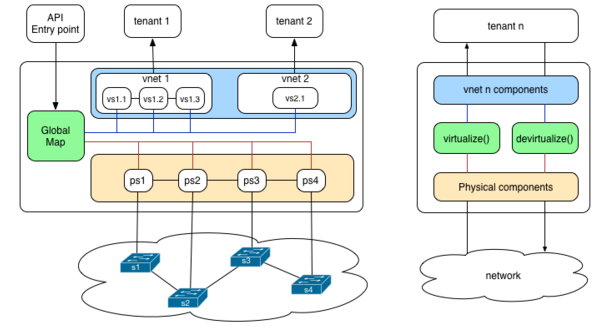
\includegraphics[width=0.7\textwidth]{logo/virtual-detail.png}
  \caption{网络虚拟化模块架构}
  \label{fig:virtual}
\end{figure}

面向网络的南向接口,主要用建立和维护与基础设施的连接,即对底层物理网络实现集中管控。管理虚拟平台和基础设施之间的OpenFlow信道。面向租户的北向接口,主要是呈现vSDN网络给租户,管理租户控制器和vSDN网络之间的OpenFlow信道。全局映射表,完成物理网络和虚拟网络之间的相互映射,并且连接这两个网络。API服务器,主要是监听JSONRPC调用系统配置和系统/网络状态信息,以此同时,租户亦可进行虚拟网络的创建、删除、修改工作。

虚拟化平台不仅拥有底层物理网络拓扑,而且还有每个租户的虚拟网络拓扑。底层的物理网络拓扑是通过虚拟化平台下发LLDP报文获取到的,而上层的虚拟网络拓扑则是由其本身生成的。即租户的控制器下发的LLDP报文不会直接送到底层物理网络,而是在虚拟化平台中通过查询底层物理拓扑,从而模拟了LLDP的过程,向上提供网络拓扑。虚拟化模块通过映射算法,解耦了底层网络和租户网络。即南向上,虚拟化模块作为控制器,接收底层物理设备的信息,并下发流表等报文到底层设备。北向上,其作为交换机集合,向租户的控制器发送OF报文。从而将一条完整的控制通路,变成了两段相互独立的控制通路。而这两者之间的映射关系,保存在映射表中。在图\ref{fig:virtual}中,蓝色部分是面向租户的,而橙色部分是面向交换机的。两者之间互不可见,即租户看不到物理的交换机数据。而绿色部分是两者结合的纽带,保存了网络映射的数据。在数据上行、下行的过程中通过查表修改的方式,翻译成正确的数据。如图\ref{fig:virtual}右侧所示,上行数据需要调用virtualize()函数,而下行数据需要调用devirtualize()函数。


\subsection{通信模块}
通信模块基于消息队列实现,消息队列是一种应用程序对应用程序的通信方法。应用程序通过读写出入队列的消息(针对应用程序的数据)来通信,而无需专用连接来链接它们。消息传递指的是程序之间通过在消息中发送数据进行通信,而不是通过直接调用彼此来通信。队列作为消息代理,给应用程序提供一个共同的平台,用于存储发送/接受的消息。直到消息从队列中被接收端收到为止。具体的通信模块如图\ref{fig:rabbitmq}所示。

\begin{figure}[!htb]
  \centering
  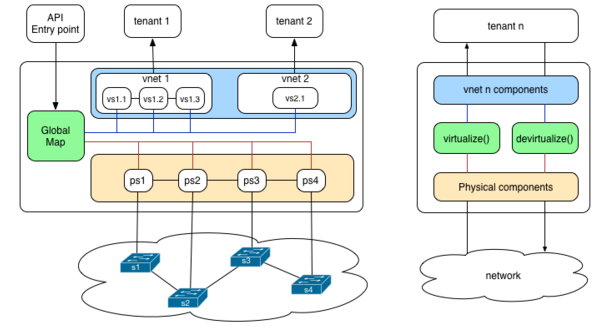
\includegraphics[width=0.7\textwidth]{logo/virtual-detail.png}
  \caption{通信模块架构图}
  \label{fig:rabbitmq}
\end{figure}

由图中可以看出,生产者绑定Exchange,Exchange是一个消息交换机,它指定消息按什么规则,路由到哪个队列。具体的路由规则由RoutingKey设定,RoutingKey作为路由关键字,Exchange根据这个关键字进行消息投递。队列用于消息的存储,直到消息被消费者从队列中读取完毕。

本文基于消息队列实现通信模块,带来诸多好处。消息队列降低了进程间的耦合度,即使一个处理消息的进程挂掉,加入队列中的消息仍然可以在系统恢复后被处理。而这种允许重试或者延后处理请求的能力保证了平台的健壮性。消息队列提供的冗余机制保证了消息能被实际的处理,只要一个进程读取了该队列即可。在此基础上,消息队列提供了一个"只送达一次"保证。无论有多少进程在从队列中领取数据,每一个消息只能被处理一次。这之所以成为可能,是因为获取一个消息只是"预定"了这个消息,暂时把它移出了队列。除非客户端明确的表示已经处理完了这个消息,否则这个消息会被放回队列中去,在一段可配置的时间之后可再次被处理。很多时候,你不想也不需要立即处理消息。消息队列提供了异步处理机制,允许你把一个消息放入队列,但并不立即处理它。你想向队列中放入多少消息就放多少,然后在你乐意的时候再去处理它们。

\subsection{控制器模块}
控制器是 SDN 的重要组成部分,其设计与实现是SDN 最为关键的技术环节之一。作为数据控制分离的
SDN 的操作系统,控制器具有举足轻重的地位,它是连接底层交换设备与上层应用的桥梁。一方面,控制器
通过南向接口协议对底层网络交换设备进行集中管理、状态监测、转发决策以处理和调度数据平面的流量:另
一方面,控制器通过北向接口向上层应用开放多个层次的可编程能力,允许网络用户根据特定的应用场景灵活
地制定各种网络策略。

本研究中,我们提供了基于Ryu控制器的Linux镜像,租户可以基于次镜像进行控制器的创建,默认情况下控制器占用TCP的6633端口。租户只需要讲自己创建的虚拟网络指向自己的SDN控制器,即可实现自由控制器对虚拟网络的集中管控。租户可以根据自身需求进行控制器北向应用的相关开发工作。本文主要实现了链路的时延、带宽的测量,以及定制化流表的下发实验。

本文选用的Ryu控制器,是由日本最大的电信服务提供商NTT主导幵发的基于Python语言的开源控制器,是一个基于组件的软件定义网络架构,是一个基于Apache协议的完全开源的SDN控制器,对于软件组件提供了良好的API接口,便于开发人员创建新的网络管理与控制中的应用,Ryu支持管理网络设备的多种网络协议,诸如:OpenFlow,Netconf,OF-config等,租户Ryu架构和主要组件如图\ref{fig:ryu}所示。OF-conf、Netconf等组件主要提供了对OpenFlow交换机的控制能力,Topology用于对SDN网络的拓扑进行管理,REST提供了上层的API接口。

\begin{figure}[!htb]
  \centering
  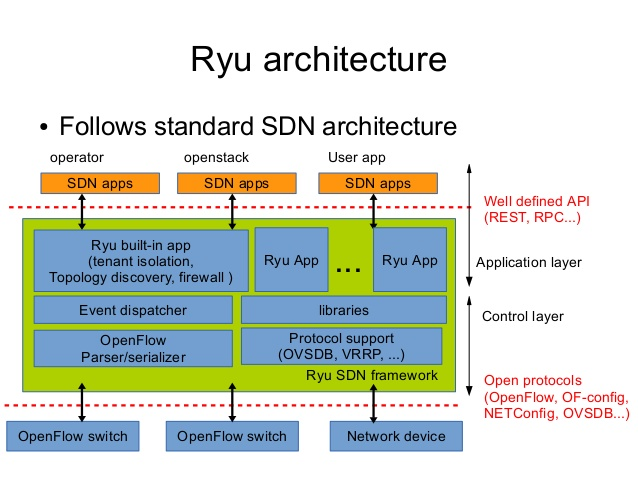
\includegraphics[width=0.7\textwidth]{logo/ryu.jpg}
  \caption{Ryu架构图}
  \label{fig:ryu}
\end{figure}

\subsection{GUI模块}
为方便用户对虚拟网络的操作,本研究为用户开放了前端GUI接口,用户可以在前端实现物理网络、虚拟网络的拓扑获取,虚拟网络的创建和删除,全局网络带宽、时延的测量,以及数据传输链路的选取等操作。开放的GUI界面,可以在用户不理解底层实现的基础上,进行便捷行的操作。

针对GUI模块,本文基于OpenStack的Horizon模块进行二次开发,为其添加了物理网络和虚拟网络显示的模块,在显示拓扑的基础上,实现虚拟网络创建、删除,以及网络负载查询等功能。

为了租户请求的安全性,我们为其添加了认证机制,在租户发出某一请求时,首先会向通过自己的户名和密码向认证模块申请token,认证成功后,会返回该用户的唯一token标识,token中包含租户的基本信息,以及租户的权限信息,如果认证失败,该次请求结束,并返回错误信息。如果成功,租户会将刚才的请求与现有的token值合并,再一次发送至后端服务器进行请求,服务器端对token验证成功后,执行相应的请求,并将请求结果返回给前端。具体的流程如图\ref{fig:credentials}所示。

\begin{figure}[!htb]
  \centering
  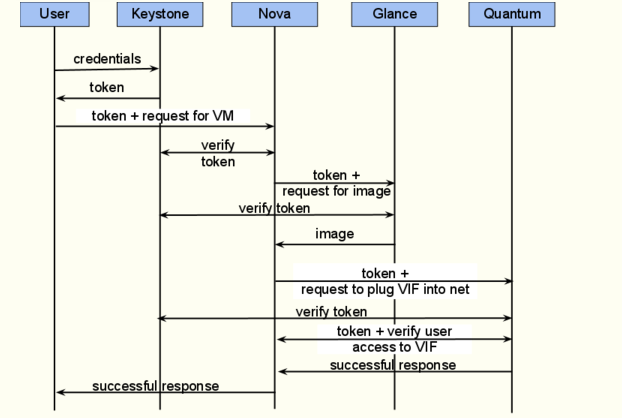
\includegraphics[width=0.7\textwidth]{logo/credentials.png}
  \caption{请求认证图}
  \label{fig:credentials}
\end{figure}

\section{本章小结}
本章主要对系统的架构做了详细的说明,为后面系统功能的实现做了铺垫。首先论文介绍了需求分析和关键技术,对本文研究内容的需求做了简要阐述,介绍了网络的虚拟化、链路负载测量、链路定制化、前端web界面的简单实现。通过对关键技术的分析说明,阐述了本文系统实现的关键点和难点,对系统搭建、链路负载测量的关键性做了分析。随后介绍了系统的整体架构图和流程图,最后对系统的各模块架构做了简单介绍,分别对网络虚拟化模块、通信模块、控制器模块、GUI模块的架构做了阐述。